% !TEX root = ../main.tex

\chapter{Results}
\label{ch:results}

\scaffold{
  Chapter purpose: the evaluation the supervisor asked to be the main part, structured from the signal chain upward: board, supply and bus, ADC noise, position noise, timing, pedal types, and finally the requirements of the proposal. Each section names its setup and conditions (also in the captions), then states what the data shows; interpretation goes to \cref{ch:discussion}. The evaluation plan of milestone~1 listed supply quality, SPI signal quality, a functional self-test, identification of known networks, accuracy and linearity, and end-to-end latency; \cref{sec:results-requirements} closes the loop on that list.
}

% !TEX root = ../main.tex

\section{Measurement Setup}
\label{sec:results-setup}

\scaffold{
  \textbf{Paragraph 1, equipment.} Oscilloscope Rigol MSO5104, laboratory supply Rigol DP932E, shown in \cref{fig:measurement-setup}; the ADCs of the board itself serve as the instrument for everything below the oscilloscope's resolution (noise, position), and the firmware logs over the debug probe for rates and state changes. Name the test points used per measurement (\cref{sec:pcb}). Give the supply voltage used for all measurements.
}

\scaffold{
  \textbf{Paragraph 2, a lesson on probes.} The first oscilloscope captures were taken with the probes on 1X. Three independent signs revealed it: floating contacts discharged with a time constant of about \qty{10}{\milli\second} (the \qty{1}{\mega\ohm} input against \qty{10}{\nano\farad}), a contact showed about \qty{150}{\pico\farad} of load, and SPI edges looked like they were driving 100 to \qty{130}{\pico\farad}. All timing and edge measurements were repeated at 10X, which loads the circuit far less \cite{tektronix2026probes}; the supply ripple measurements are taken at 1X on purpose, for the lower noise floor. State this in two sentences as part of the method, not as an apology.
}

\begin{figure}[htbp]
  \centering
  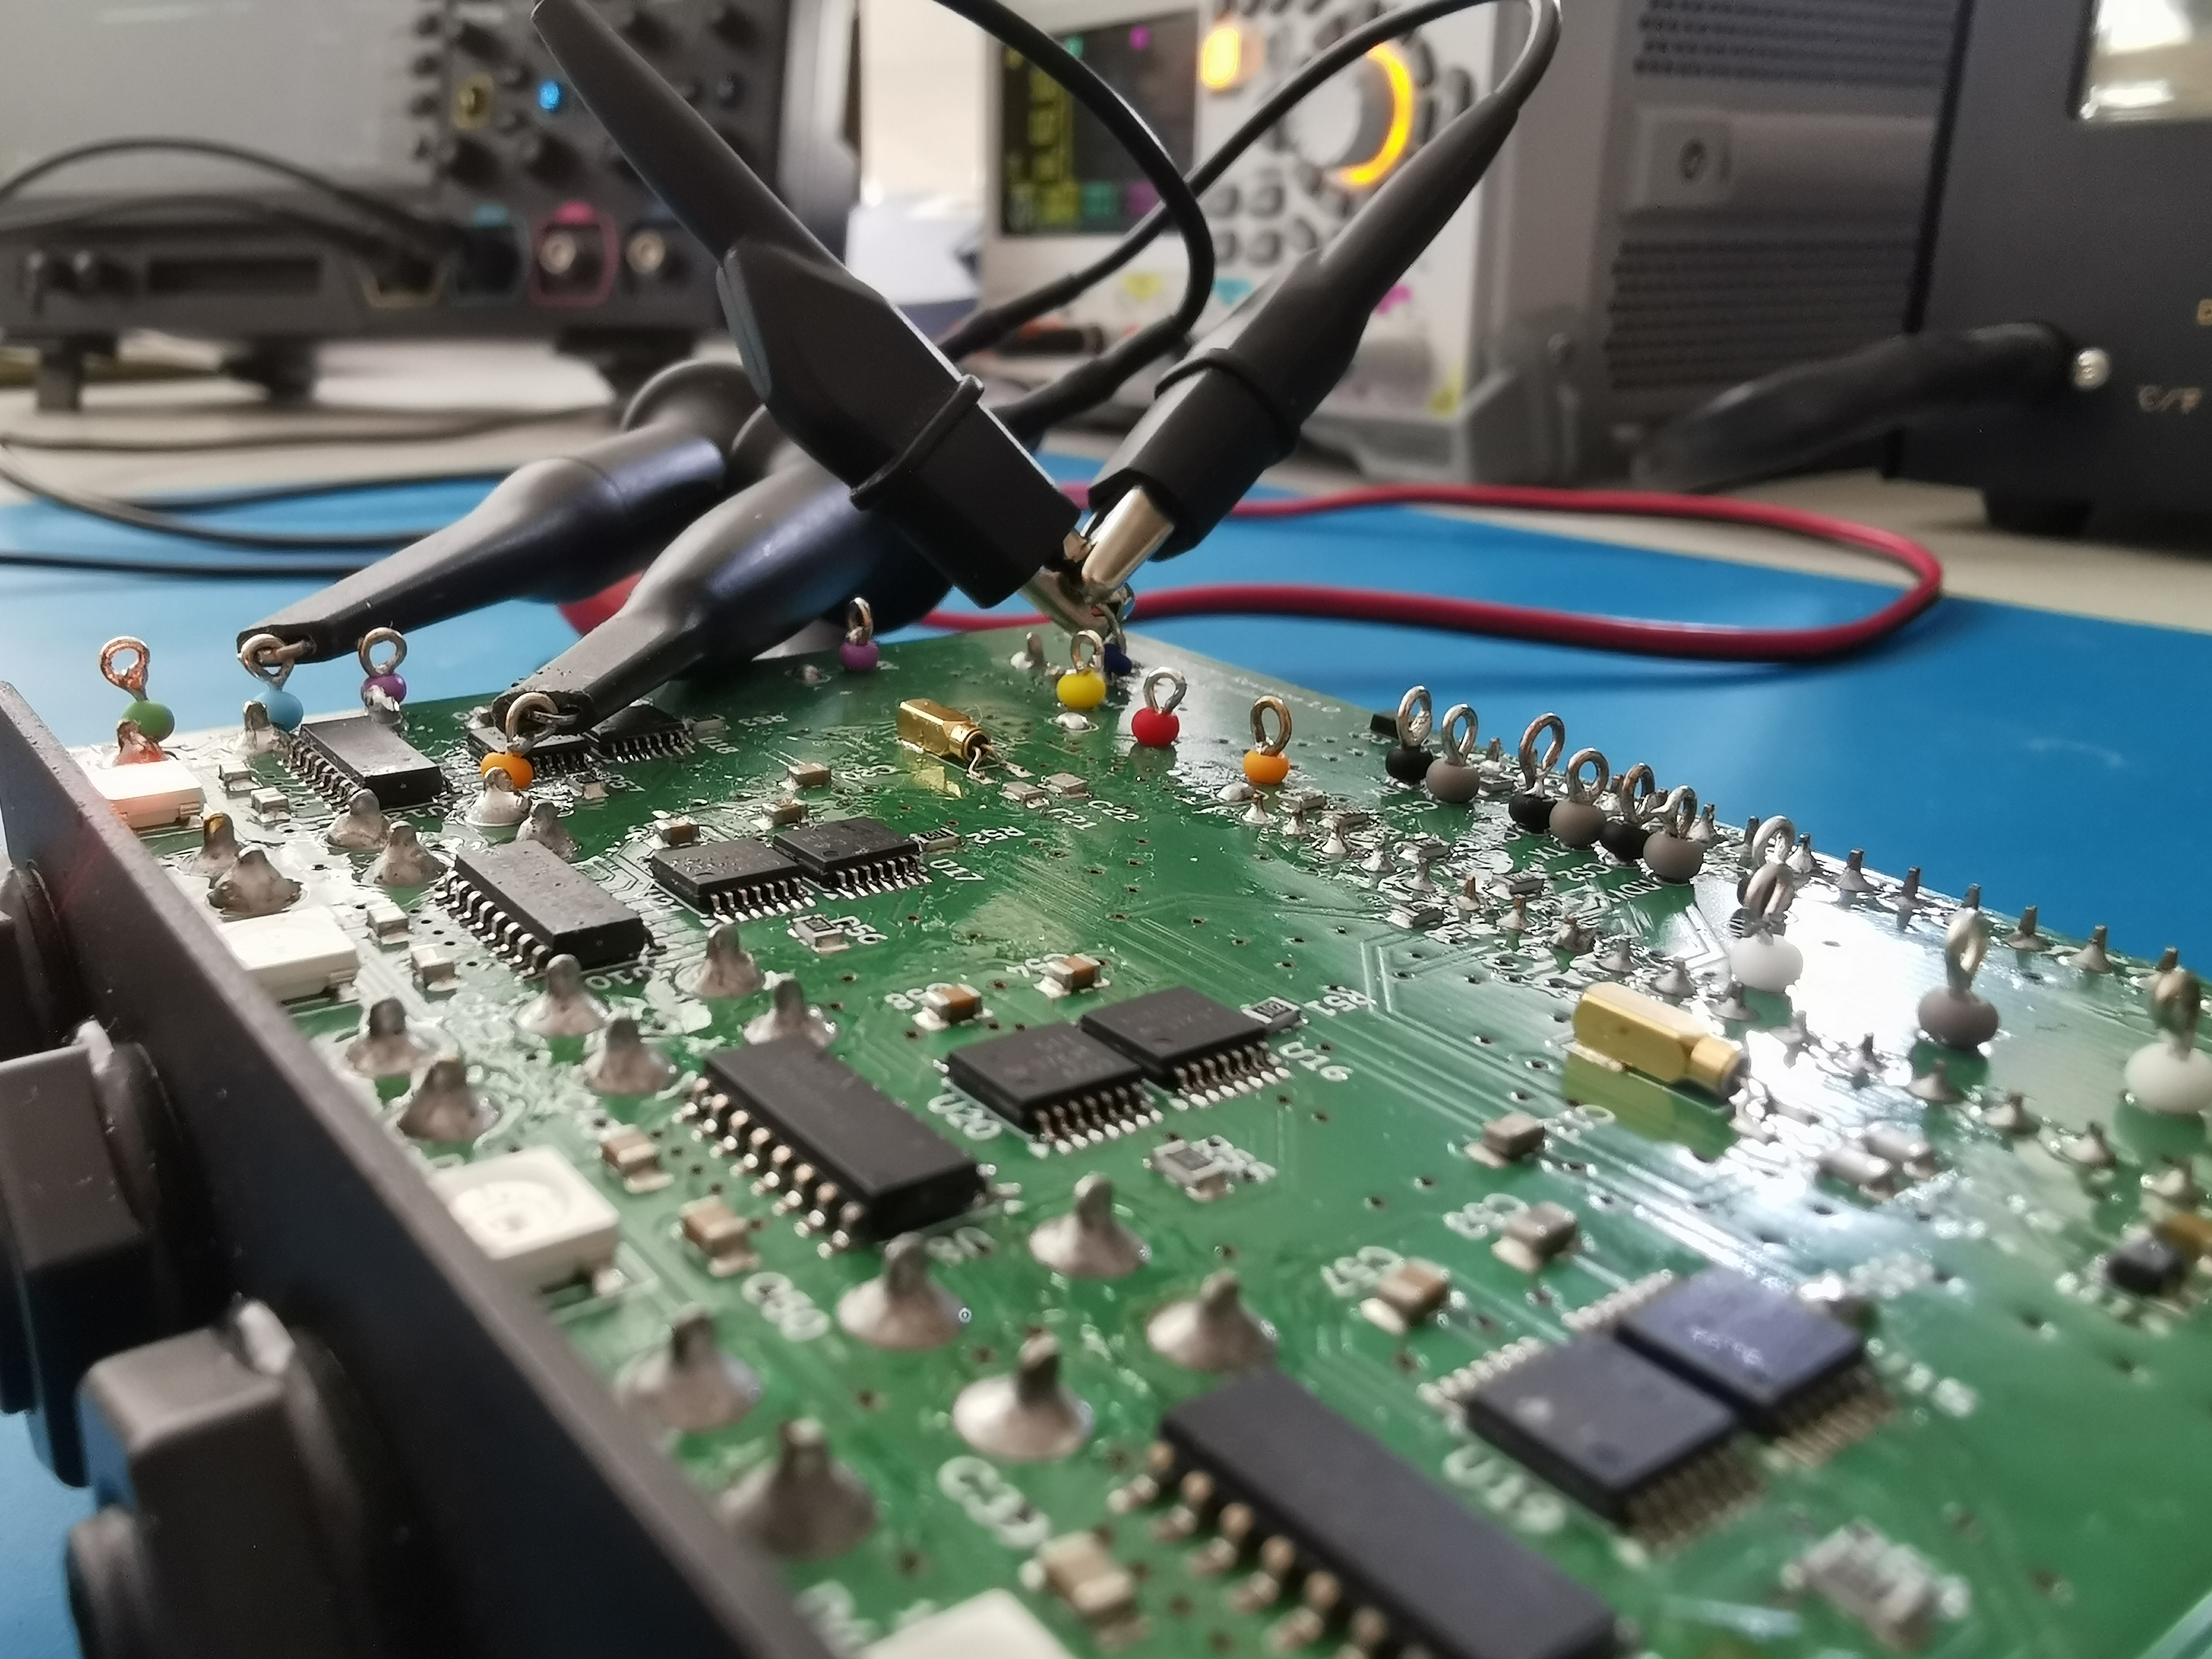
\includegraphics[width=0.75\linewidth]{05-results/figures/measurement-setup}
  \titledcaption{Measurement Setup}{\scaffoldinline{Name the board, the probes and their test points, the pedal and the instruments visible in the photo.}}
  \label{fig:measurement-setup}
\end{figure}

\openquestion{Supply voltage of the measurements}{
  Give the input voltage set on the DP932E for the measurements and the probe model used.
}

% !TEX root = ../main.tex

\section{Board Self-Test}
\label{sec:results-self-test}

\scaffold{
  \textbf{Paragraph 1, procedure.} The self-test program reads the grounded input AIN6 and the reference input AIN10 of both ADCs, then pulls every contact of every jack up and down in turn with all jacks empty and checks that exactly the ADC input that \code{board.rs} assigns to that contact follows: 4 jacks $\times$ 4 contacts $\times$ 2 polarities = 32 checks, plus the check that the tip switch follows the tip while no plug is inserted. Both ADCs convert in parallel; the whole test takes \qty{1.26}{\second}.
}

\scaffold{
  \textbf{Paragraph 2, result.} On its first run on the assembled board, every contact read \qty{2.50}{\volt} pulled up and \qty{0.0}{\volt} pulled down on exactly the expected input, which confirms switch polarity, the order of the shift-register chain and the bit mapping; the grounded inputs read \qty{0.0}{\volt} and the reference inputs \qty{2.50}{\volt}. (At that time the jacks were not yet soldered, so the tip-switch check was repeated afterwards and passed.) Present the result as \cref{tab:self-test}. Conclude in one sentence that wiring, switches, shift registers and both ADCs work as designed, which every later measurement rests on.
}

\begin{table}[htbp]
  \centering
  \titledcaption{Self-Test Result}{\scaffoldinline{Explain rows and columns and that \enquote{pass} means only the expected input followed. Fill in from a fresh run of \code{cargo run --bin detect\_pin\_mapping} with the jacks unplugged; the numbers shown are from the log of the first run.}}
  \label{tab:self-test}
  \begin{tabular}{@{}lcccc@{}}
    \toprule
    & \textbf{Tip} & \textbf{Ring} & \textbf{Sleeve} & \textbf{Tip switch} \\
    \midrule
    Jack 1 (J5) & pass & pass & pass & pass \\
    Jack 2 (J4) & pass & pass & pass & pass \\
    Jack 3 (J3) & pass & pass & pass & pass \\
    Jack 4 (J2) & pass & pass & pass & pass \\
    \midrule
    \multicolumn{5}{@{}l}{Grounded input AIN6: \qty{0.0}{\volt} on both ADCs; reference input AIN10: \qty{2.50}{\volt}} \\
    \bottomrule
  \end{tabular}
\end{table}

\openquestion{Self-test log}{
  The table is reconstructed from a development session. Rerun the self-test on the final firmware and fill in the measured values (pulled-up and pulled-down voltage per contact, AIN6 and AIN10 per ADC).
}

% !TEX root = ../main.tex

\section{Supply Rail Ripple}
\label{sec:results-supply}

\scaffold{
  \textbf{Paragraph 1, setup.} The ripple of the input (VEXT, TP15) and the three rails (TP12--TP14) was measured AC-coupled at 1X in four operating states: without microcontroller, idle or detecting, following a pedal, and following with WiFi active. Per rail and state, the RMS value averaged over 70 to 1000 acquisitions at \qty{10}{\milli\second}/div (high-resolution mode) is reported; captures at \qty{1}{\micro\second}/div reached the oscilloscope's own noise at every rail and are not shown. The noise floor of the oscilloscope, \qty{0.34}{\milli\volt} RMS, was taken under the same settings. The values were read from the oscilloscope's statistics by a script and checked by hand.
}

\scaffold{
  \textbf{Paragraph 2, the limit.} Derive the ripple that would just disturb a stable 7-bit value, drawn in \cref{fig:supply-ripple}: one MIDI step of the \qty{2.5}{\volt} reference is $\qty{2.5}{\volt}/128 = \qty{19.5}{\milli\volt}$, and requiring $\pm 3\sigma$ of Gaussian noise to fit into one step gives $\qty{19.5}{\milli\volt}/6 = \qty{3.26}{\milli\volt}$ RMS. Use the same step as \cref{sec:results-position} (1/127 of the span); the plot divides by 128, a difference below \qty{1}{\percent} that should still be made consistent in \code{create\_plots.py}. One sentence on why this is conservative: the reading is ratiometric, so ripple common to the pull rail and the reference cancels further.
}

\begin{figure}[htbp]
  \centering
  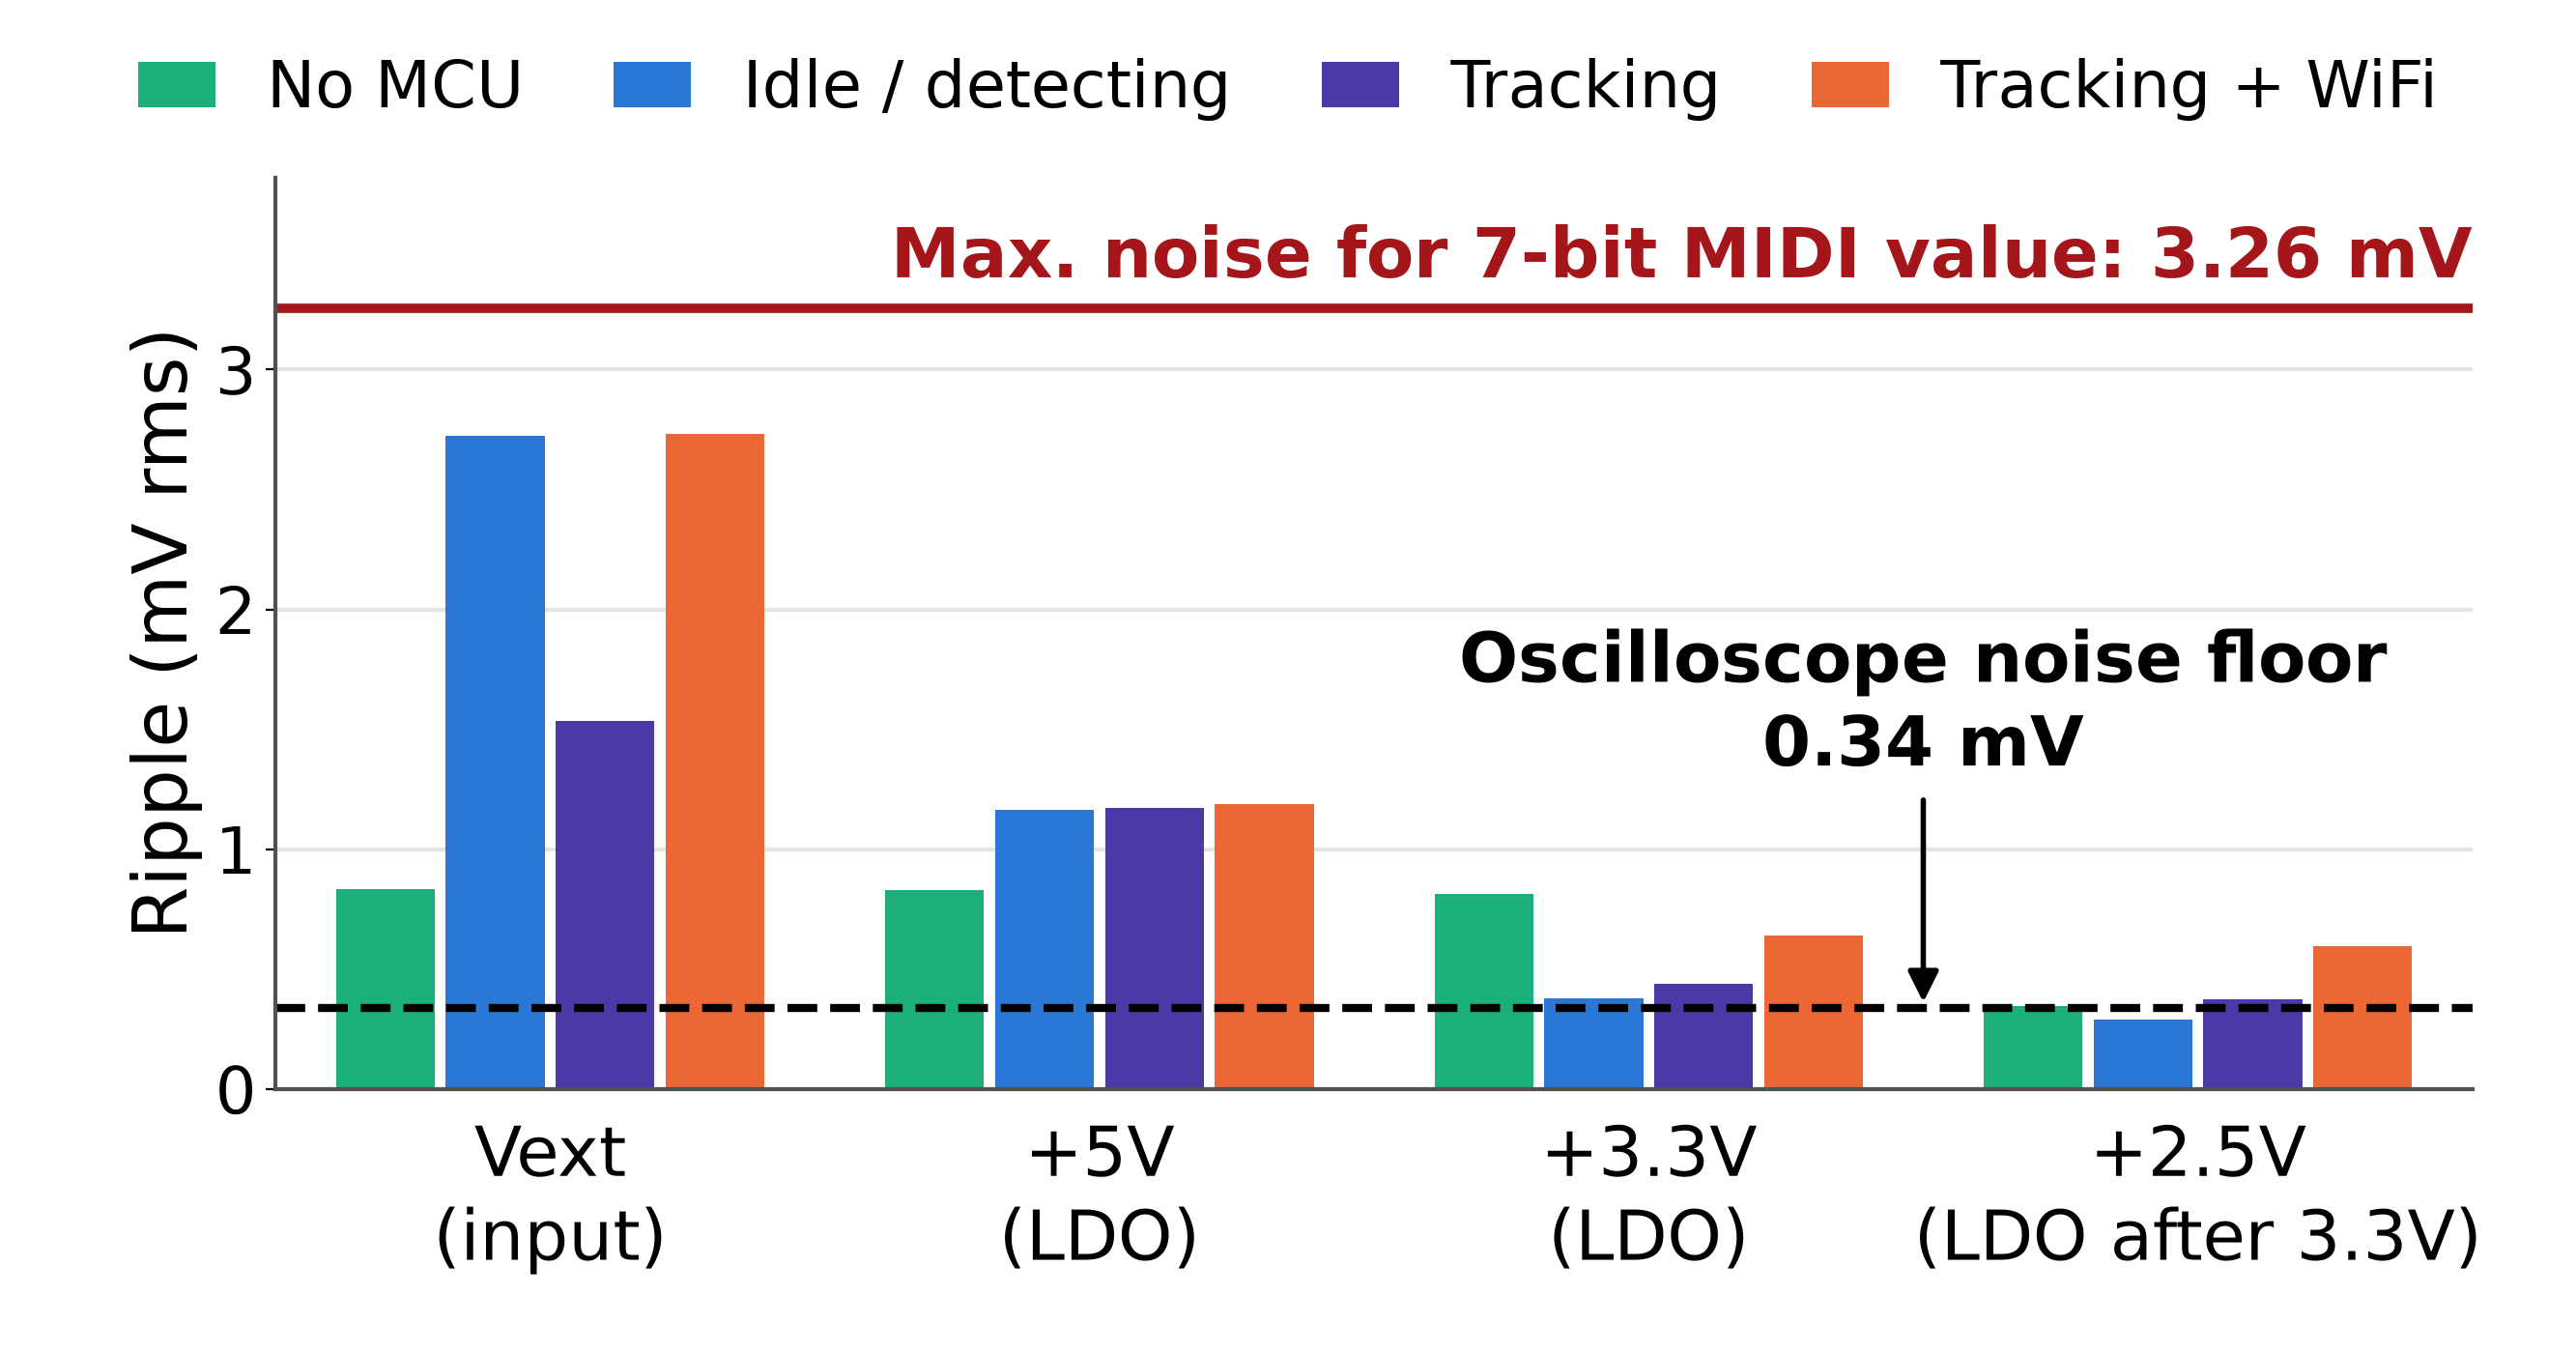
\includegraphics[width=\linewidth]{05-results/figures/supply-rail-ripple}
  \titledcaption{Supply Rail Ripple}{\scaffoldinline{State the conditions (AC coupling, 1X probe, \qty{10}{\milli\second}/div, RMS average), name the four operating states, the oscilloscope noise floor and the limit for a stable 7-bit value. Rails are ordered along the regulator chain. Source: \code{measurements/create\_plots.py}, data \code{measurements/supply\_rail\_measurement.xlsx}.}}
  \label{fig:supply-ripple}
\end{figure}

\scaffold{
  \textbf{Paragraph 3, what the data shows.} The input ripple rises from \qty{0.83}{\milli\volt} without microcontroller to about \qty{2.7}{\milli\volt} RMS once the microcontroller runs; read the exact values per state from the plot, which shows the state \enquote{idle / detecting} as high as \enquote{tracking + WiFi} and \enquote{tracking} lower, and explain or flag this. Every regulator stage lowers it, and the \qty{3.3}{\volt} and \qty{2.5}{\volt} rails stay between 0.3 and \qty{0.6}{\milli\volt}, at or just above the noise floor, so their exact values are not meaningful. WiFi is the only state that visibly raises them. The \qty{5}{\volt} rail shows about \qty{1.2}{\milli\volt} RMS but about \qty{16}{\milli\volt} peak-to-peak once the microcontroller runs, i.e. short spikes rather than broadband noise. Every rail stays below the \qty{3.26}{\milli\volt} limit; the \qty{2.5}{\volt} rail by a factor of about five even with WiFi.
}

\openquestion{Supply data quality}{
  Three readings without microcontroller (VEXT, \qty{5}{\volt}, \qty{3.3}{\volt}) were taken without resetting the oscilloscope statistics between rails, which makes the \qty{3.3}{\volt} rail look worse without the microcontroller than with it. Decide whether to remeasure, mark or drop them. Confirm that the noise floor capture (image~2) was taken with the probe tip on the ground pad, and give the cause of the spikes on the \qty{5}{\volt} rail if known (suspected: the switching regulator of the Pico module).
}

% !TEX root = ../main.tex

\section{SPI Signal Integrity}
\label{sec:results-spi}

\scaffold{
  \textbf{Paragraph 1, timing and content.} Captures of SPI0 at TP5--TP9 show a clock of \qty{3.95}{\mega\hertz} (the system clock of \qty{150}{\mega\hertz} divided by 38 for the requested \qty{4}{\mega\hertz}), SPI mode~0, and chip-select guards of \qty{9.8}{\micro\second} and \qty{11.45}{\micro\second} for the configured \qty{10}{\micro\second}. One data-register read takes \qty{30.65}{\micro\second} with the chip selected, of which \qty{9.4}{\micro\second} is clocking; decoding the bits gives the read command \code{0x44} followed by a 24-bit result. State that the guards dominate a transaction but are negligible against the \qty{4}{\milli\second} conversion time of a reading.
}

\scaffold{
  \textbf{Paragraph 2, edges.} \Cref{fig:spi-edges} shows clock and data edges captured at 10X: rise times of \qty{10.2}{\nano\second} (clock) and \qty{11.2}{\nano\second} (data), fall time \qty{8.4}{\nano\second}, overshoot within one oscilloscope step (\qty{40}{\milli\volt}), no ringing. The data line changes on the falling clock edge and is sampled on the rising one, so it is stable for about \qty{127}{\nano\second} on either side; a \qty{10}{\nano\second} edge uses about \qty{8}{\percent} of the half period. The edges are slowed on purpose by the \qty{47}{\ohm} series resistors. Two notes for honesty: the first capture at 1X showed edges of 24 to \qty{27}{\nano\second}, which was the probe's load; and the 10X capture was averaged, which supports \enquote{no ringing} but says nothing about one-off glitches.
}

\begin{figure}[htbp]
  \centering
  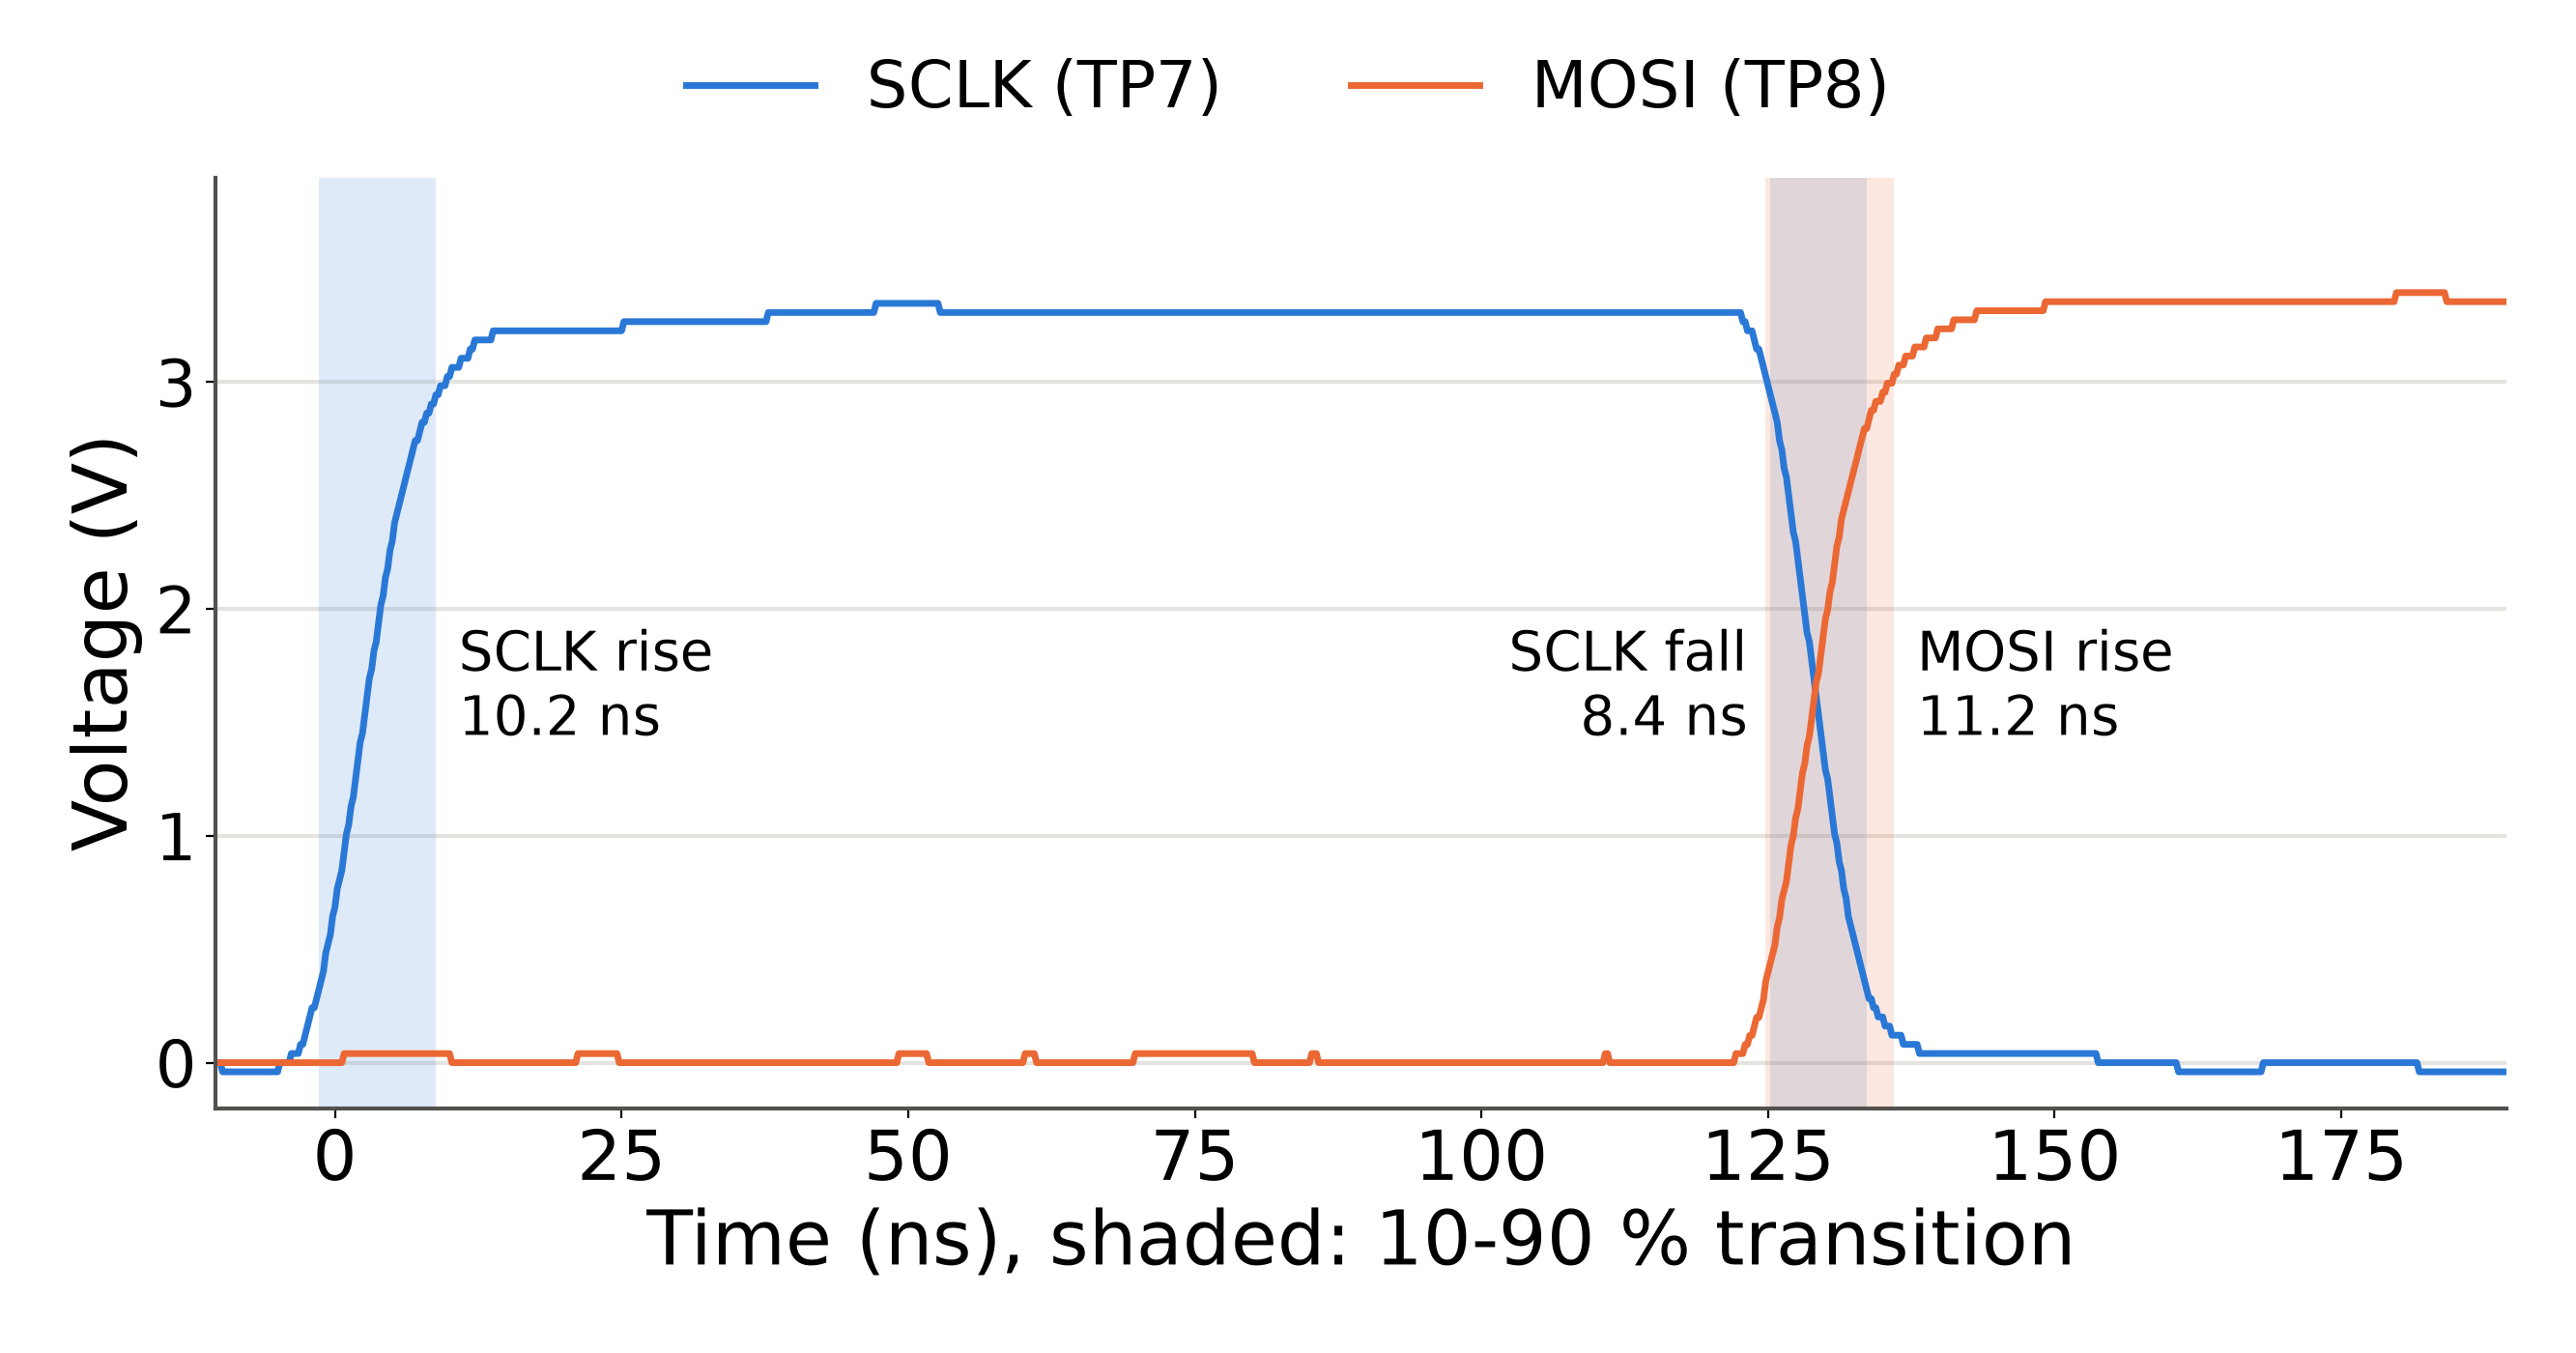
\includegraphics[width=0.85\linewidth]{05-results/figures/spi-edges}
  \titledcaption{SPI Edges}{\scaffoldinline{State conditions (10X probes, SCLK at TP7, MOSI at TP8, averaged capture) and that the shaded bands are the 10 to \qty{90}{\percent} transitions with their durations. Source: \code{measurements/create\_plots.py}, data \code{spi\_edges\_rise.csv}.}}
  \label{fig:spi-edges}
\end{figure}

\scaffold{
  \textbf{Paragraph 3, error-free transfer.} Firmware-side check: at \qty{4}{\mega\hertz} with a \qty{10}{\micro\second} guard, 300 consecutive readings contained no outlying code (more than six robust standard deviations from the median), where the breadboard had produced flipped bits at \qty{4}{\mega\hertz} and needed \qty{50}{\micro\second}.
}

% !TEX root = ../main.tex

\section{ADC Noise on the PCB}
\label{sec:results-adc-noise}

\scaffold{
  \textbf{Paragraph 1, setup.} The capture program held every contact in one drive state (pulled low, pulled high, or floating) and recorded all inputs for \qty{30}{\second} at \qty{315}{\hertz}, bipolar coding; this was the first measurement on the assembled board, before the operating point of \cref{sec:update-rate} was chosen. Present \cref{tab:adc-noise}.
}

\begin{table}[htbp]
  \centering
  \titledcaption{ADC Noise on the Empty Board}{\scaffoldinline{State conditions (\qty{315}{\hertz}, \qty{30}{\second} per state, all jacks empty) and that ranges span the inputs of both ADCs.}}
  \label{tab:adc-noise}
  \begin{tabular}{@{}llll@{}}
    \toprule
    \textbf{Input} & \textbf{Mean} & \textbf{Noise ($\sigma$)} & \textbf{Drift in \qty{30}{\second}} \\
    \midrule
    Contacts pulled low & \qty{+1.3}{\milli\volt} / \qty{+1.5}{\milli\volt} & 15 to \qty{23}{\micro\volt} & $\leq \qty{0.04}{\milli\volt}$ \\
    Contacts pulled high & \qtyrange{2.4998}{2.5001}{\volt} & 50 to \qty{60}{\micro\volt} & $\leq \qty{0.16}{\milli\volt}$ \\
    Grounded input AIN6 & \qty{+1.3}{\milli\volt} / \qty{+1.5}{\milli\volt} & 15 to \qty{21}{\micro\volt} & none \\
    Reference input AIN10 & \qtyrange{2.4999}{2.5000}{\volt} & 55 to \qty{85}{\micro\volt} & $\leq \qty{0.17}{\milli\volt}$ \\
    \bottomrule
  \end{tabular}
\end{table}

\scaffold{
  \textbf{Paragraph 2, what it shows.} The noise is about \qty{20}{\micro\volt} near ground and about \qty{55}{\micro\volt} near the rail; the part that grows with the voltage most likely comes from the reference and cancels in the ratiometric reading. The constant offset of about \qty{1.4}{\milli\volt} appears on the grounded input as well, so it belongs to the ADC, not to the switches, and the measured rails of \cref{sec:pair-measurement} compensate it. Floating inputs drift by tenths of a volt, charged by about \qty{0.2}{\nano\ampere} to \qty{0.5}{\nano\ampere} of leakage into the filter capacitors, which through a pedal of \qty{100}{\kilo\ohm} or less amounts to less than \qty{50}{\micro\volt}. Compare with the breadboard (about \qty{1}{\milli\volt}) in half a sentence.
}

\scaffold{
  \textbf{Paragraph 3, with a pedal.} With the \qty{10.85}{\kilo\ohm} pedal reproducing the three solver pairs, driven contacts read 0.03 to \qty{0.12}{\milli\volt} and the floating contact up to \qty{0.36}{\milli\volt} where it reads the wiper directly, part of it slow wander attributed to the wiper contact. This set the solver's noise figure first to \qty{0.4}{\milli\volt} at \qty{315}{\hertz}, later to \qty{0.5}{\milli\volt} at \qty{819}{\hertz} (\cref{tab:adc-characterization}).
}

% !TEX root = ../main.tex

\section{Position Noise and Accuracy}
\label{sec:results-position}

\scaffold{
  \textbf{Paragraph 1, position noise.} With the \qty{10.85}{\kilo\ohm} pedal held still, the position solved at \qty{819}{\hertz} has a standard deviation of \num{274} parts per million of travel (\cref{tab:conditioning-fix}). One MIDI step is $1/127$, \num{7874} parts per million, so the jitter is about 1/29 of a step, and the emitted 7-bit value does not change. In the following mode, where only the wiper is read, the single-reading noise of \num{203} parts per million (\cref{tab:adc-characterization}) applies. State the consequence plainly: the limit of the output resolution is the 7-bit MIDI value, not the measurement.
}

\begin{figure}[htbp]
  \centering
  \placeholderfigure{
    \textbf{Content.} (a) Histogram of a few thousand positions of a pedal held still in the following mode, x axis in parts per million of travel around the mean, with the width of one MIDI step (\num{7874} ppm) drawn on the same axis; (b) the emitted MIDI value over the same time, a flat line.
    \textbf{Focus.} The ratio between the width of the histogram and one MIDI step.
    \textbf{How to obtain.} Log the raw position of one jack over the debug probe (\code{defmt}) for about \qty{30}{\second} while the pedal is still, plot with \code{measurements/create\_plots.py}. This measurement (M3 of the measurement plan) has not been made yet.
  }
  \titledcaption{Position Noise}{\scaffoldinline{Conditions (pedal, position, rate, duration, number of samples) and the meaning of the drawn MIDI step.}}
  \label{fig:position-noise}
\end{figure}

\scaffold{
  \textbf{Paragraph 2, accuracy against known networks.} The milestone plan promised a sweep of precision resistors against the measured ratio and the identification of known static networks, including shorted and open arms. State what exists: the solver's arithmetic is verified against simulated networks by 25 host tests, including every short and open case; and the identified total of the test pedal was repeatable (\num{10.844} to \qty{10.850}{\kilo\ohm} over 300 solves); its agreement with an independent measurement, for example an ohmmeter across ring and sleeve, is not recorded. If the measurement with known resistors is made, present it here as measured against actual arm resistance with the relative error, and the error of the total against the total, with the prediction of \cref{tab:pull-resistance}.
}

\openquestion{Accuracy and linearity measurement}{
  No measurement with precision resistors or a decade box (identification of known networks, ratio sweep for linearity) is in the repository, although the milestone plan promised it. Was it made? If not, say so in the text and in \cref{sec:results-requirements}, with the reason. At least compare the identified totals of the real pedals with an ohmmeter reading.
}

% !TEX root = ../main.tex

\section{Recognition Time}
\label{sec:results-recognition}

\scaffold{
  \textbf{Paragraph 1, setup.} Channel~1 on the tip switch and channel~2 on the ring of one jack, 10X probes, trigger on the tip switch rising through \qty{1.9}{\volt} (the plug lifting it), \qty{500}{\milli\second} window, at least 1~million points. The drive pattern of the jack changes with every state, so the ring voltage shows the phases of the jack monitor directly: the latch edges of the shift register mark where one phase ends and the next begins. The switch into following is not visible, because following keeps the drives of the last pair; it is inferred as one pair length (\qty{14.6}{\milli\second}) after the last edge. Five plug-ins and three unplugs were captured.
}

\scaffold{
  \textbf{Paragraph 2, plug-in with fresh rails.} Walk through \cref{fig:plug-in-fresh} along its labelled phases: waiting for the next plug check, the three pairs (ring pulled low at \qty{0.28}{\volt}, floating at the star point, pulled high), then following. Present \cref{tab:plug-in}: the plug was noticed 4.9 to \qty{47.3}{\milli\second} after insertion, as expected from a check every \qty{50}{\milli\second}; identification took 44 to \qty{48}{\milli\second}; in total 65 to \qty{95}{\milli\second}. A pair sometimes takes \qty{18.8}{\milli\second} instead of \qty{14.7}{\milli\second}, one extra conversion for the plug check of the other jack on the same ADC. The first run is a useful edge case: the plug was noticed before it was fully seated, tip and ring were shorted, the first pair was rejected and repeated, and the result was still correct after \qty{65}{\milli\second}.
}

\begin{figure}[htbp]
  \centering
  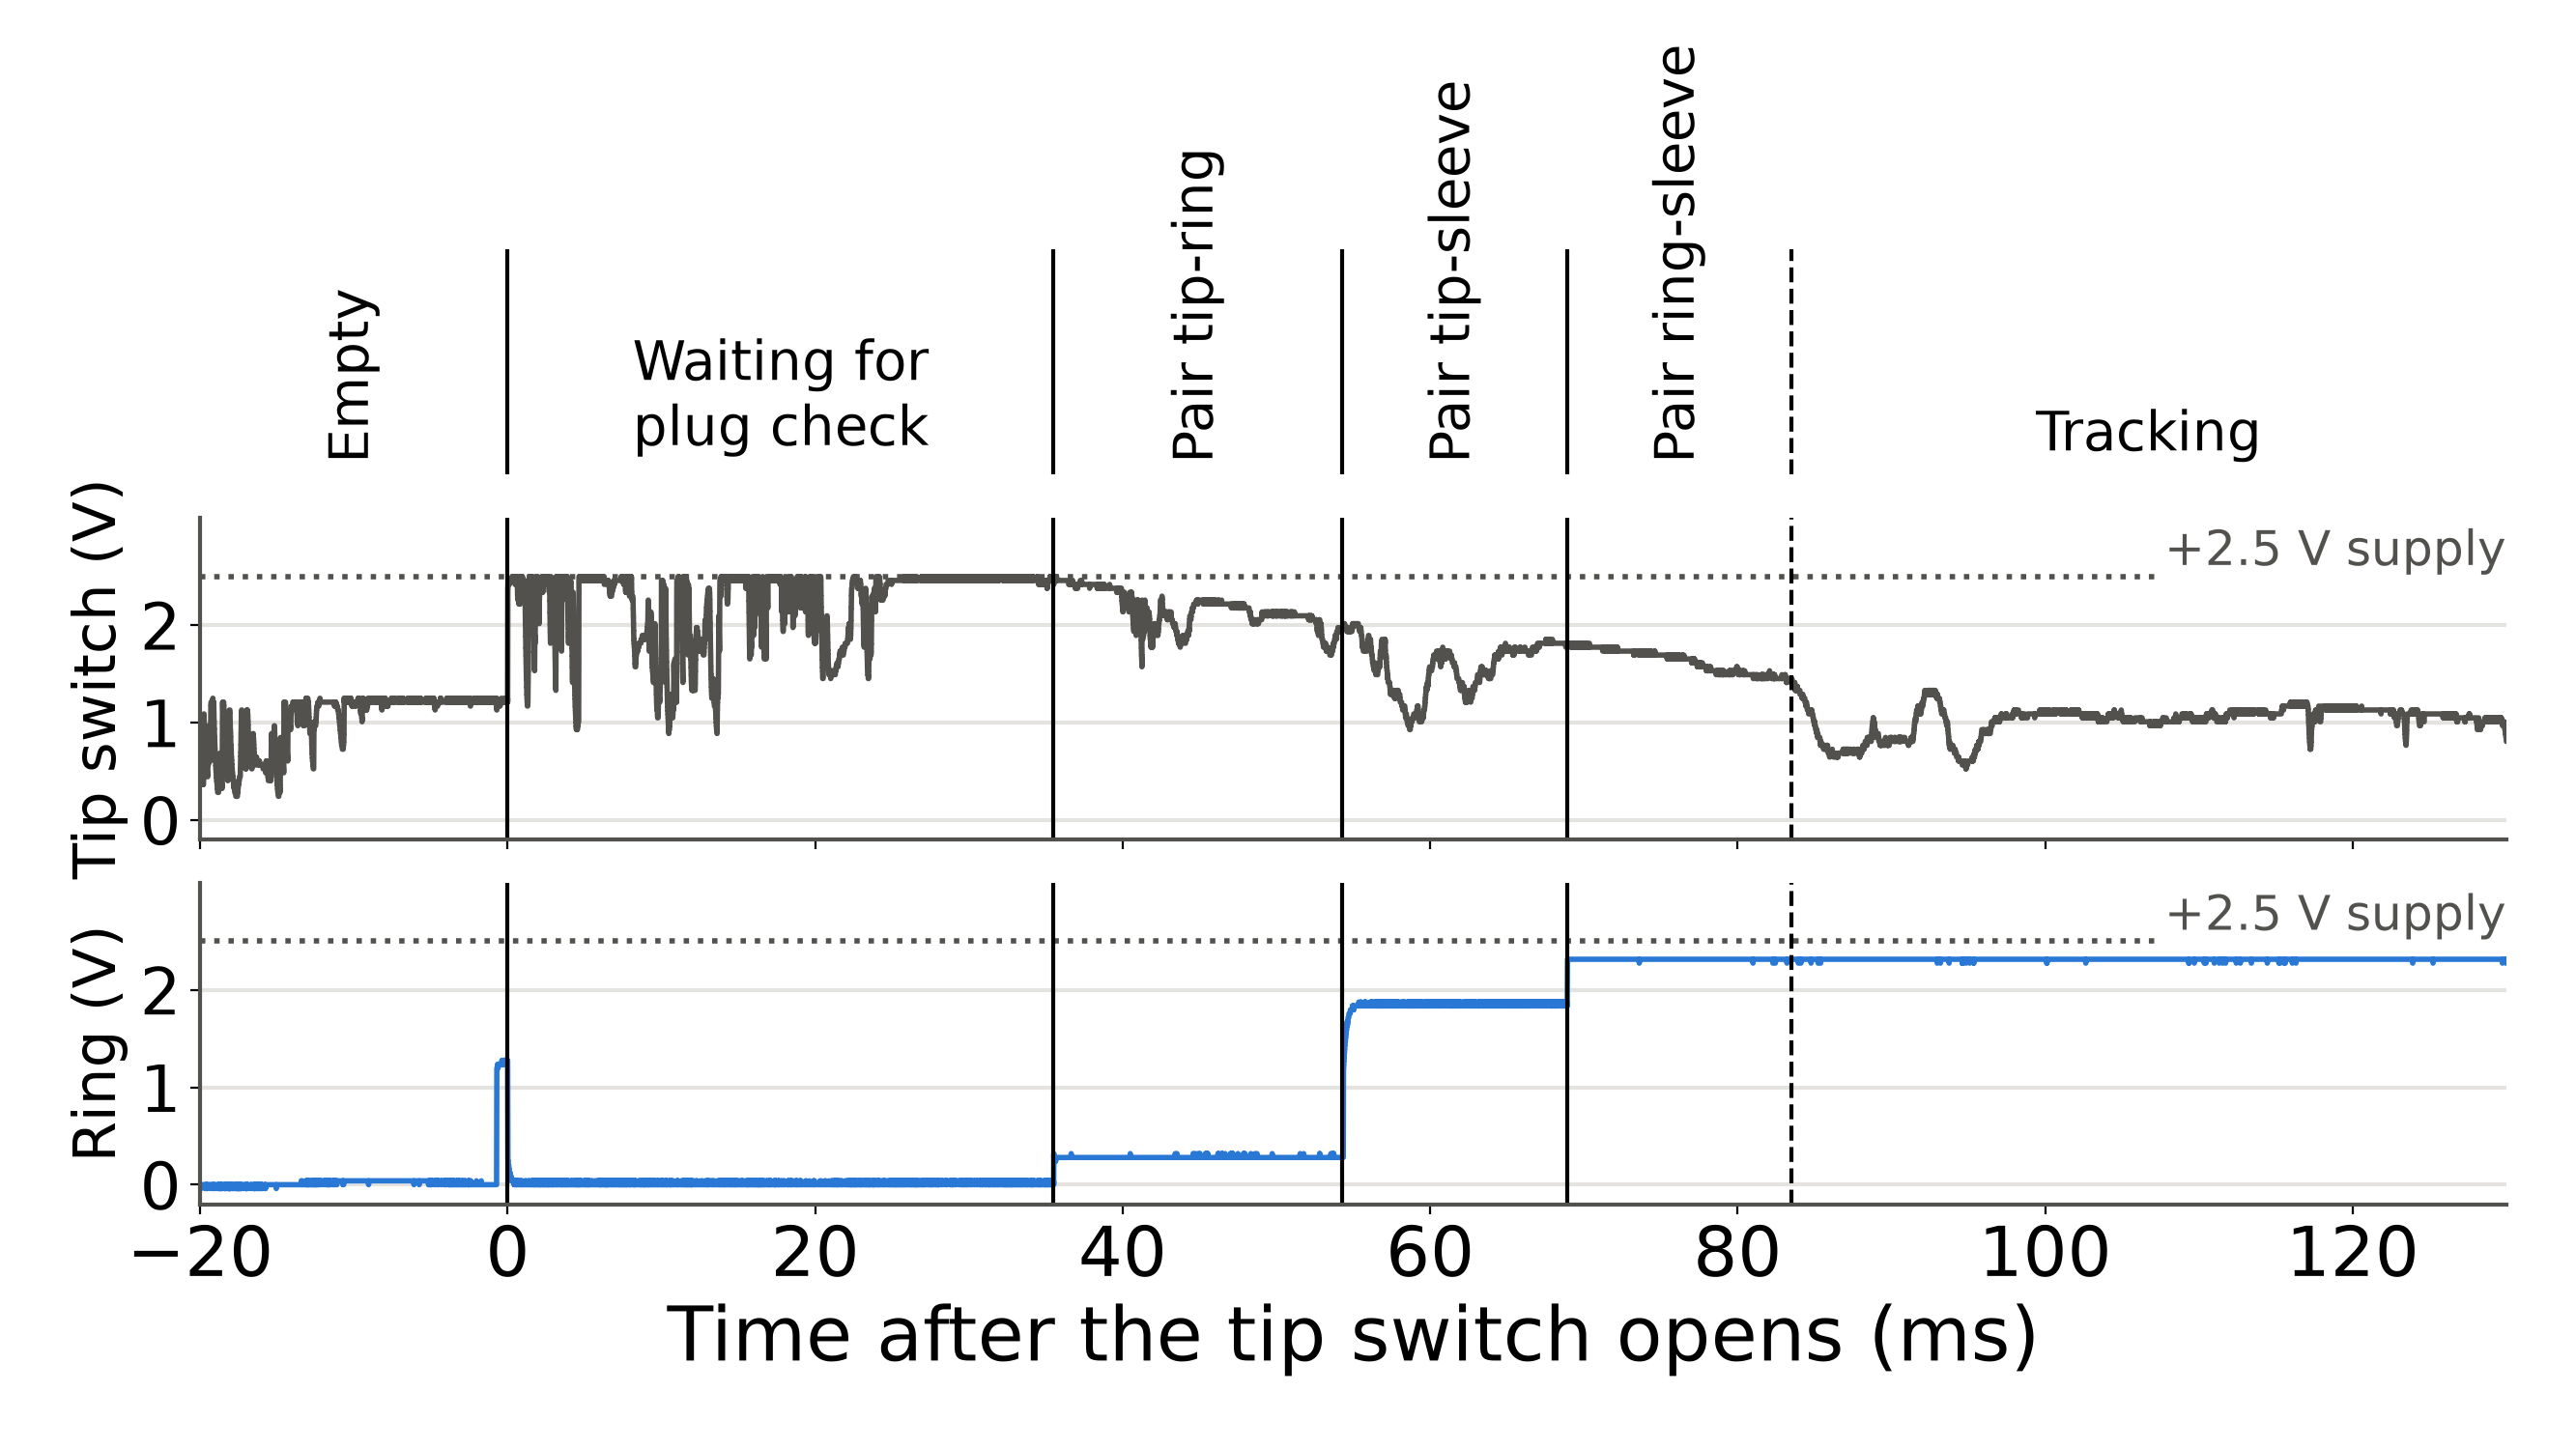
\includegraphics[width=\linewidth]{05-results/figures/plug-in-fresh-rails}
  \titledcaption{Plug-In with Fresh Rails}{\scaffoldinline{Conditions (tip switch and ring of jack~1, 10X, trigger on the tip switch at \qty{1.9}{\volt}, rails measured less than \qty{30}{\second} before); the vertical lines are latch edges, the dashed one is inferred. Capture \code{plugin5.csv}; source \code{measurements/create\_plots.py}.}}
  \label{fig:plug-in-fresh}
\end{figure}

\begin{table}[htbp]
  \centering
  \titledcaption{Plug-In Timing}{\scaffoldinline{Times in milliseconds after the tip switch opened, except the column \enquote{first pair}, which gives its duration; the start of following is inferred as the last latch plus one pair length.}}
  \label{tab:plug-in}
  \begin{tabular}{@{}lrrrr@{}}
    \toprule
    \textbf{Run} & \textbf{Plug noticed} & \textbf{First pair} & \textbf{Last latch} & \textbf{Following} \\
    \midrule
    1 & 4.9 & 31.2 (repeated) & 50.9 & $\approx$ 65 \\
    2 & 47.3 & 18.8 & 80.7 & $\approx$ 95 \\
    3 & 45.6 & 14.7 & 75.0 & $\approx$ 90 \\
    4 & 17.6 & 18.9 & 51.1 & $\approx$ 66 \\
    5 & 35.5 & 18.8 & 68.9 & $\approx$ 84 \\
    \midrule
    Rails older than \qty{30}{\second} & 49.4 & 14.7 & 292.7 & $\approx$ 300 \\
    \bottomrule
  \end{tabular}
\end{table}

\scaffold{
  \textbf{Paragraph 3, plug-in with a rail refresh.} The rails are re-measured before a solve if they are older than \qty{30}{\second}. \Cref{fig:plug-in-refresh} shows this worst case: the plug check came just before the insertion (\qty{49.4}{\milli\second} of waiting), the rails took \qty{213.8}{\milli\second} (48 readings of \qty{4.45}{\milli\second}, all arms high, then all low), and the pairs about \qty{30}{\milli\second} to \qty{44}{\milli\second}: about \qty{300}{\milli\second} in total. Mention that the pair voltages of this run differ from the other five because the wiper contact resistance changed between the pairs, and that the solver still accepted the result.
}

\begin{figure}[htbp]
  \centering
  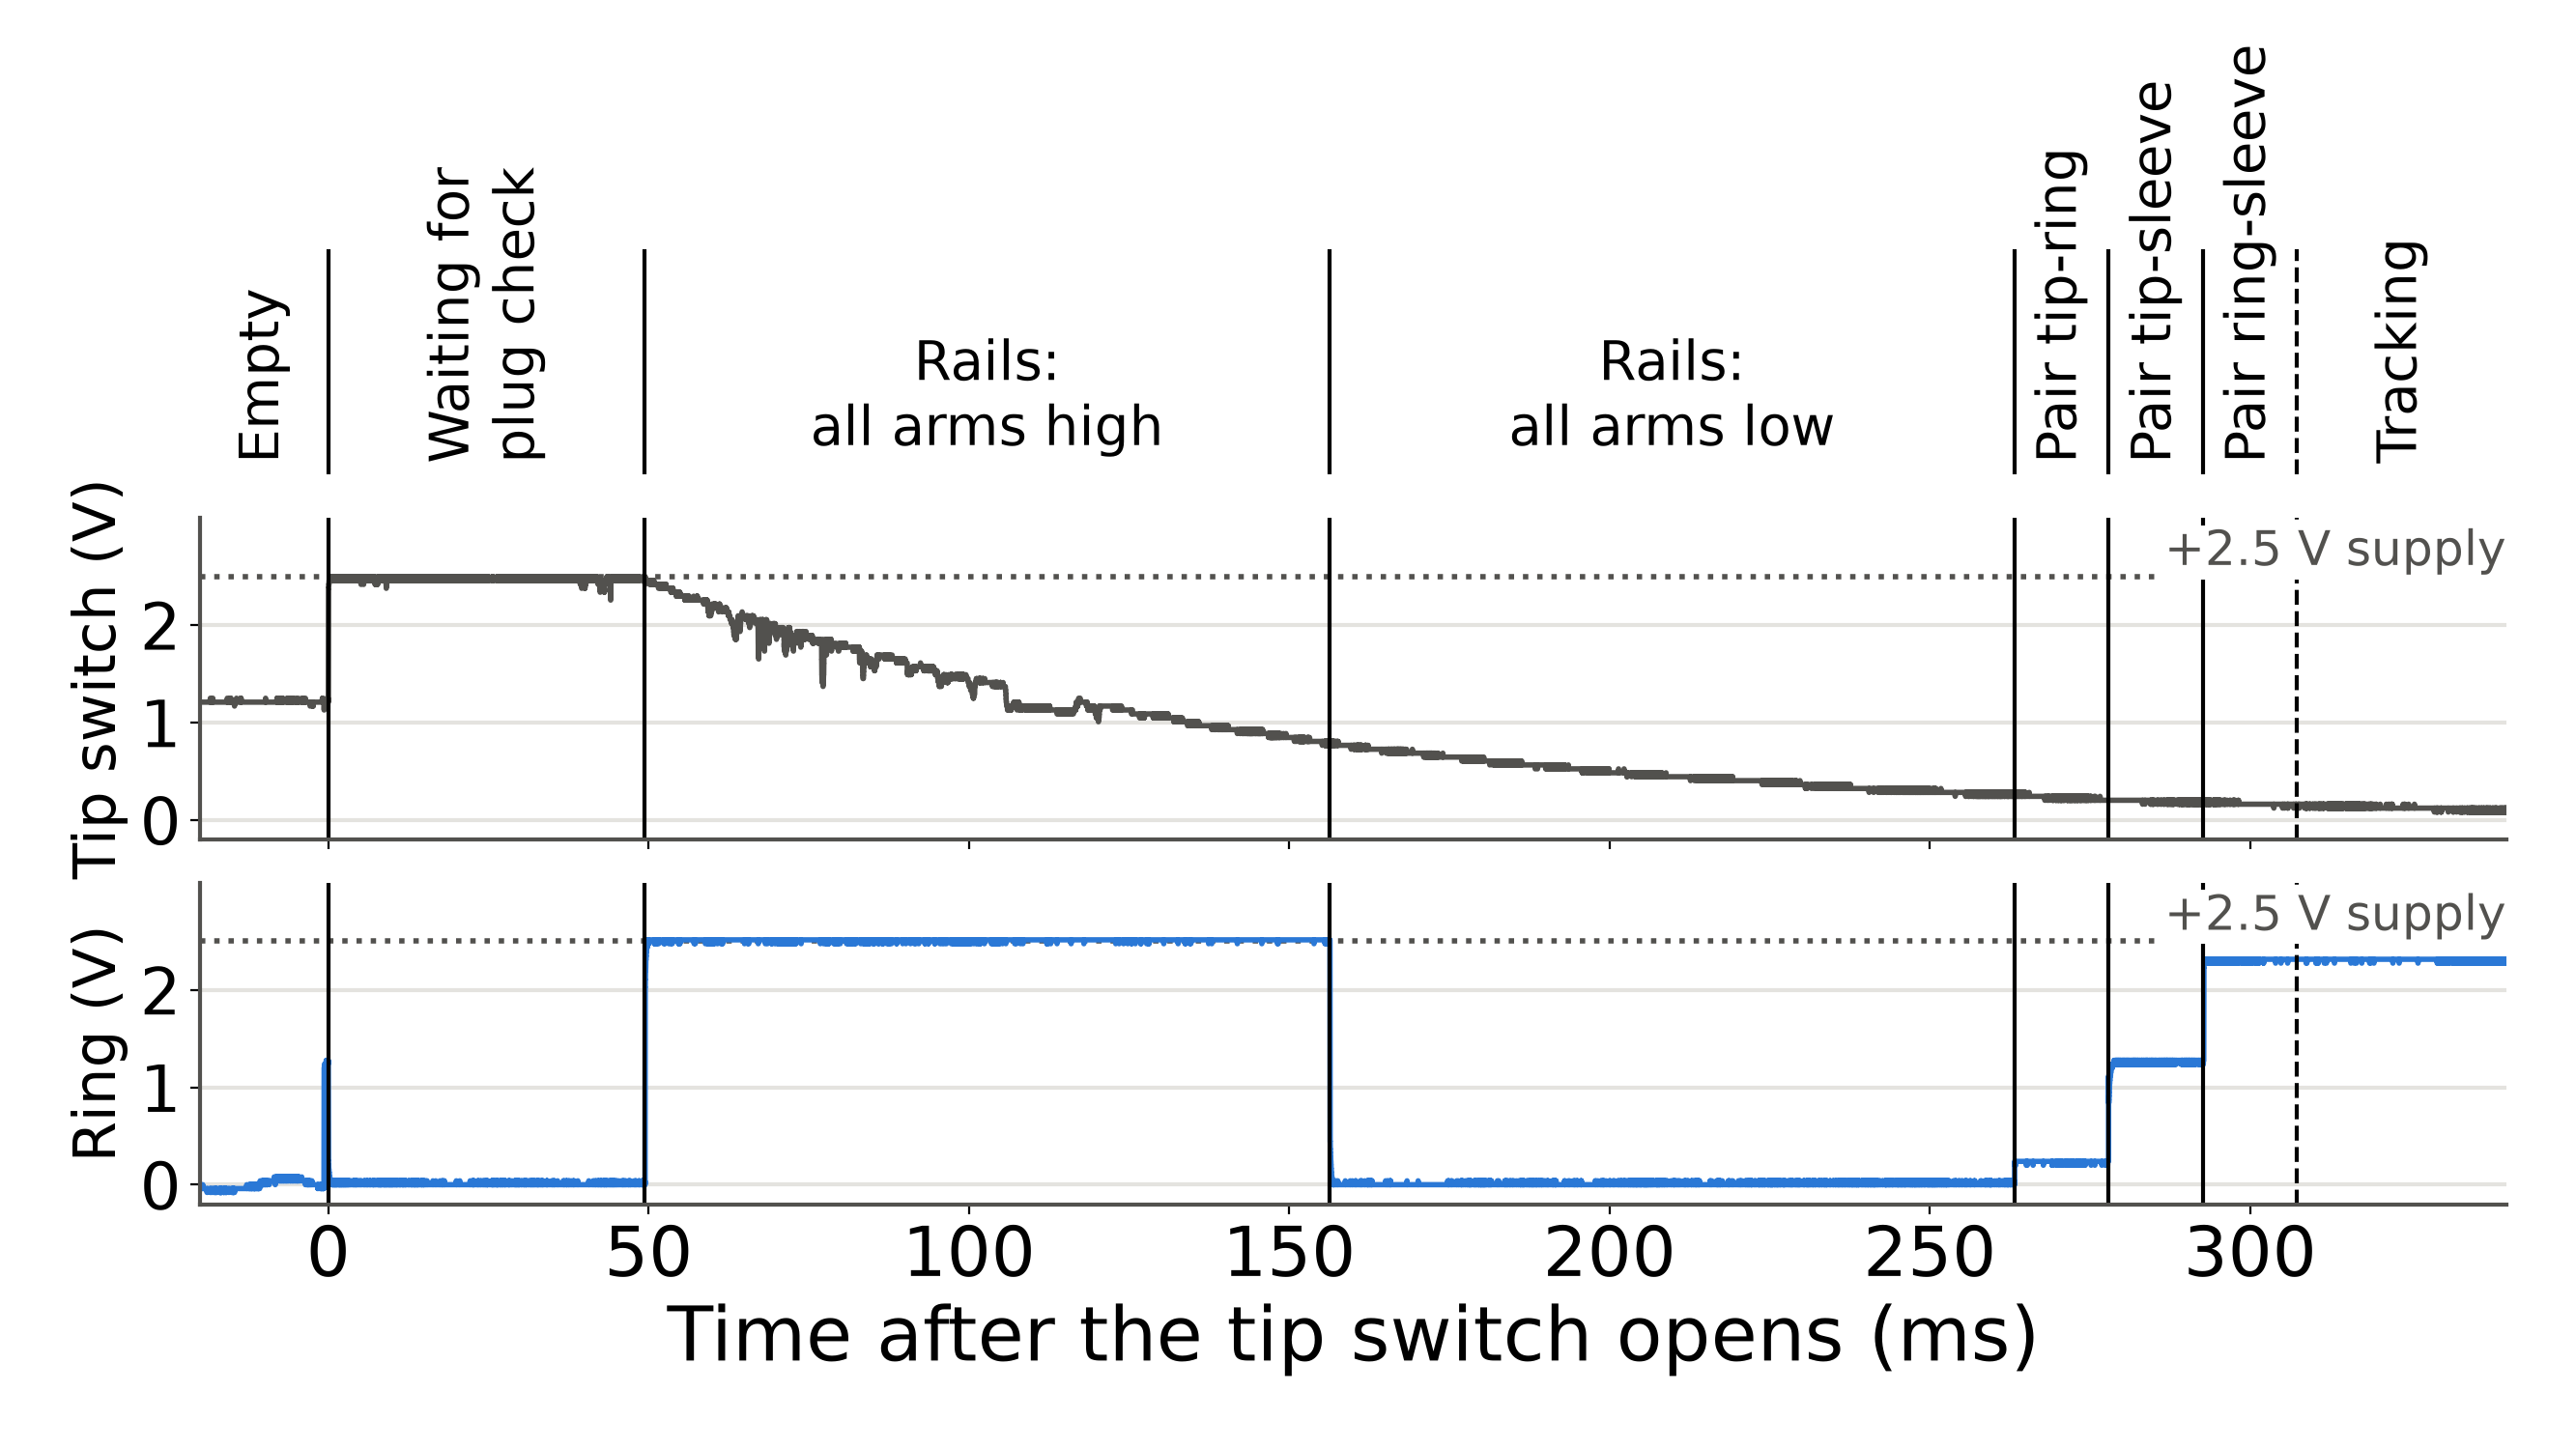
\includegraphics[width=\linewidth]{05-results/figures/plug-in-rail-refresh}
  \titledcaption{Plug-In with Rail Refresh}{\scaffoldinline{Same conditions as \cref{fig:plug-in-fresh}, but the rails were older than \qty{30}{\second}; name the two rail phases. Capture \code{plugin\_w\_rail\_meas.csv}.}}
  \label{fig:plug-in-refresh}
\end{figure}

\scaffold{
  \textbf{Paragraph 4, unplug.} \Cref{fig:unplug} (trigger on the tip switch closing): the ring loses the pedal's current about \qty{2}{\milli\second} before the tip switch closes; the firmware drops the pedal 2 to \qty{27}{\milli\second} later, re-measures the rails (about \qty{214}{\milli\second}, since the pedal had been followed for longer than \qty{30}{\second}), solves, finds no current, and the plug check reports the jack empty after 260, 330 and \qty{391}{\milli\second} in the three runs. In two of three runs a second solve was needed, because the first one saw a current just above the conduction threshold. Conclude that the rail refresh dominates both the worst-case plug-in and the unplug time.
}

\begin{figure}[htbp]
  \centering
  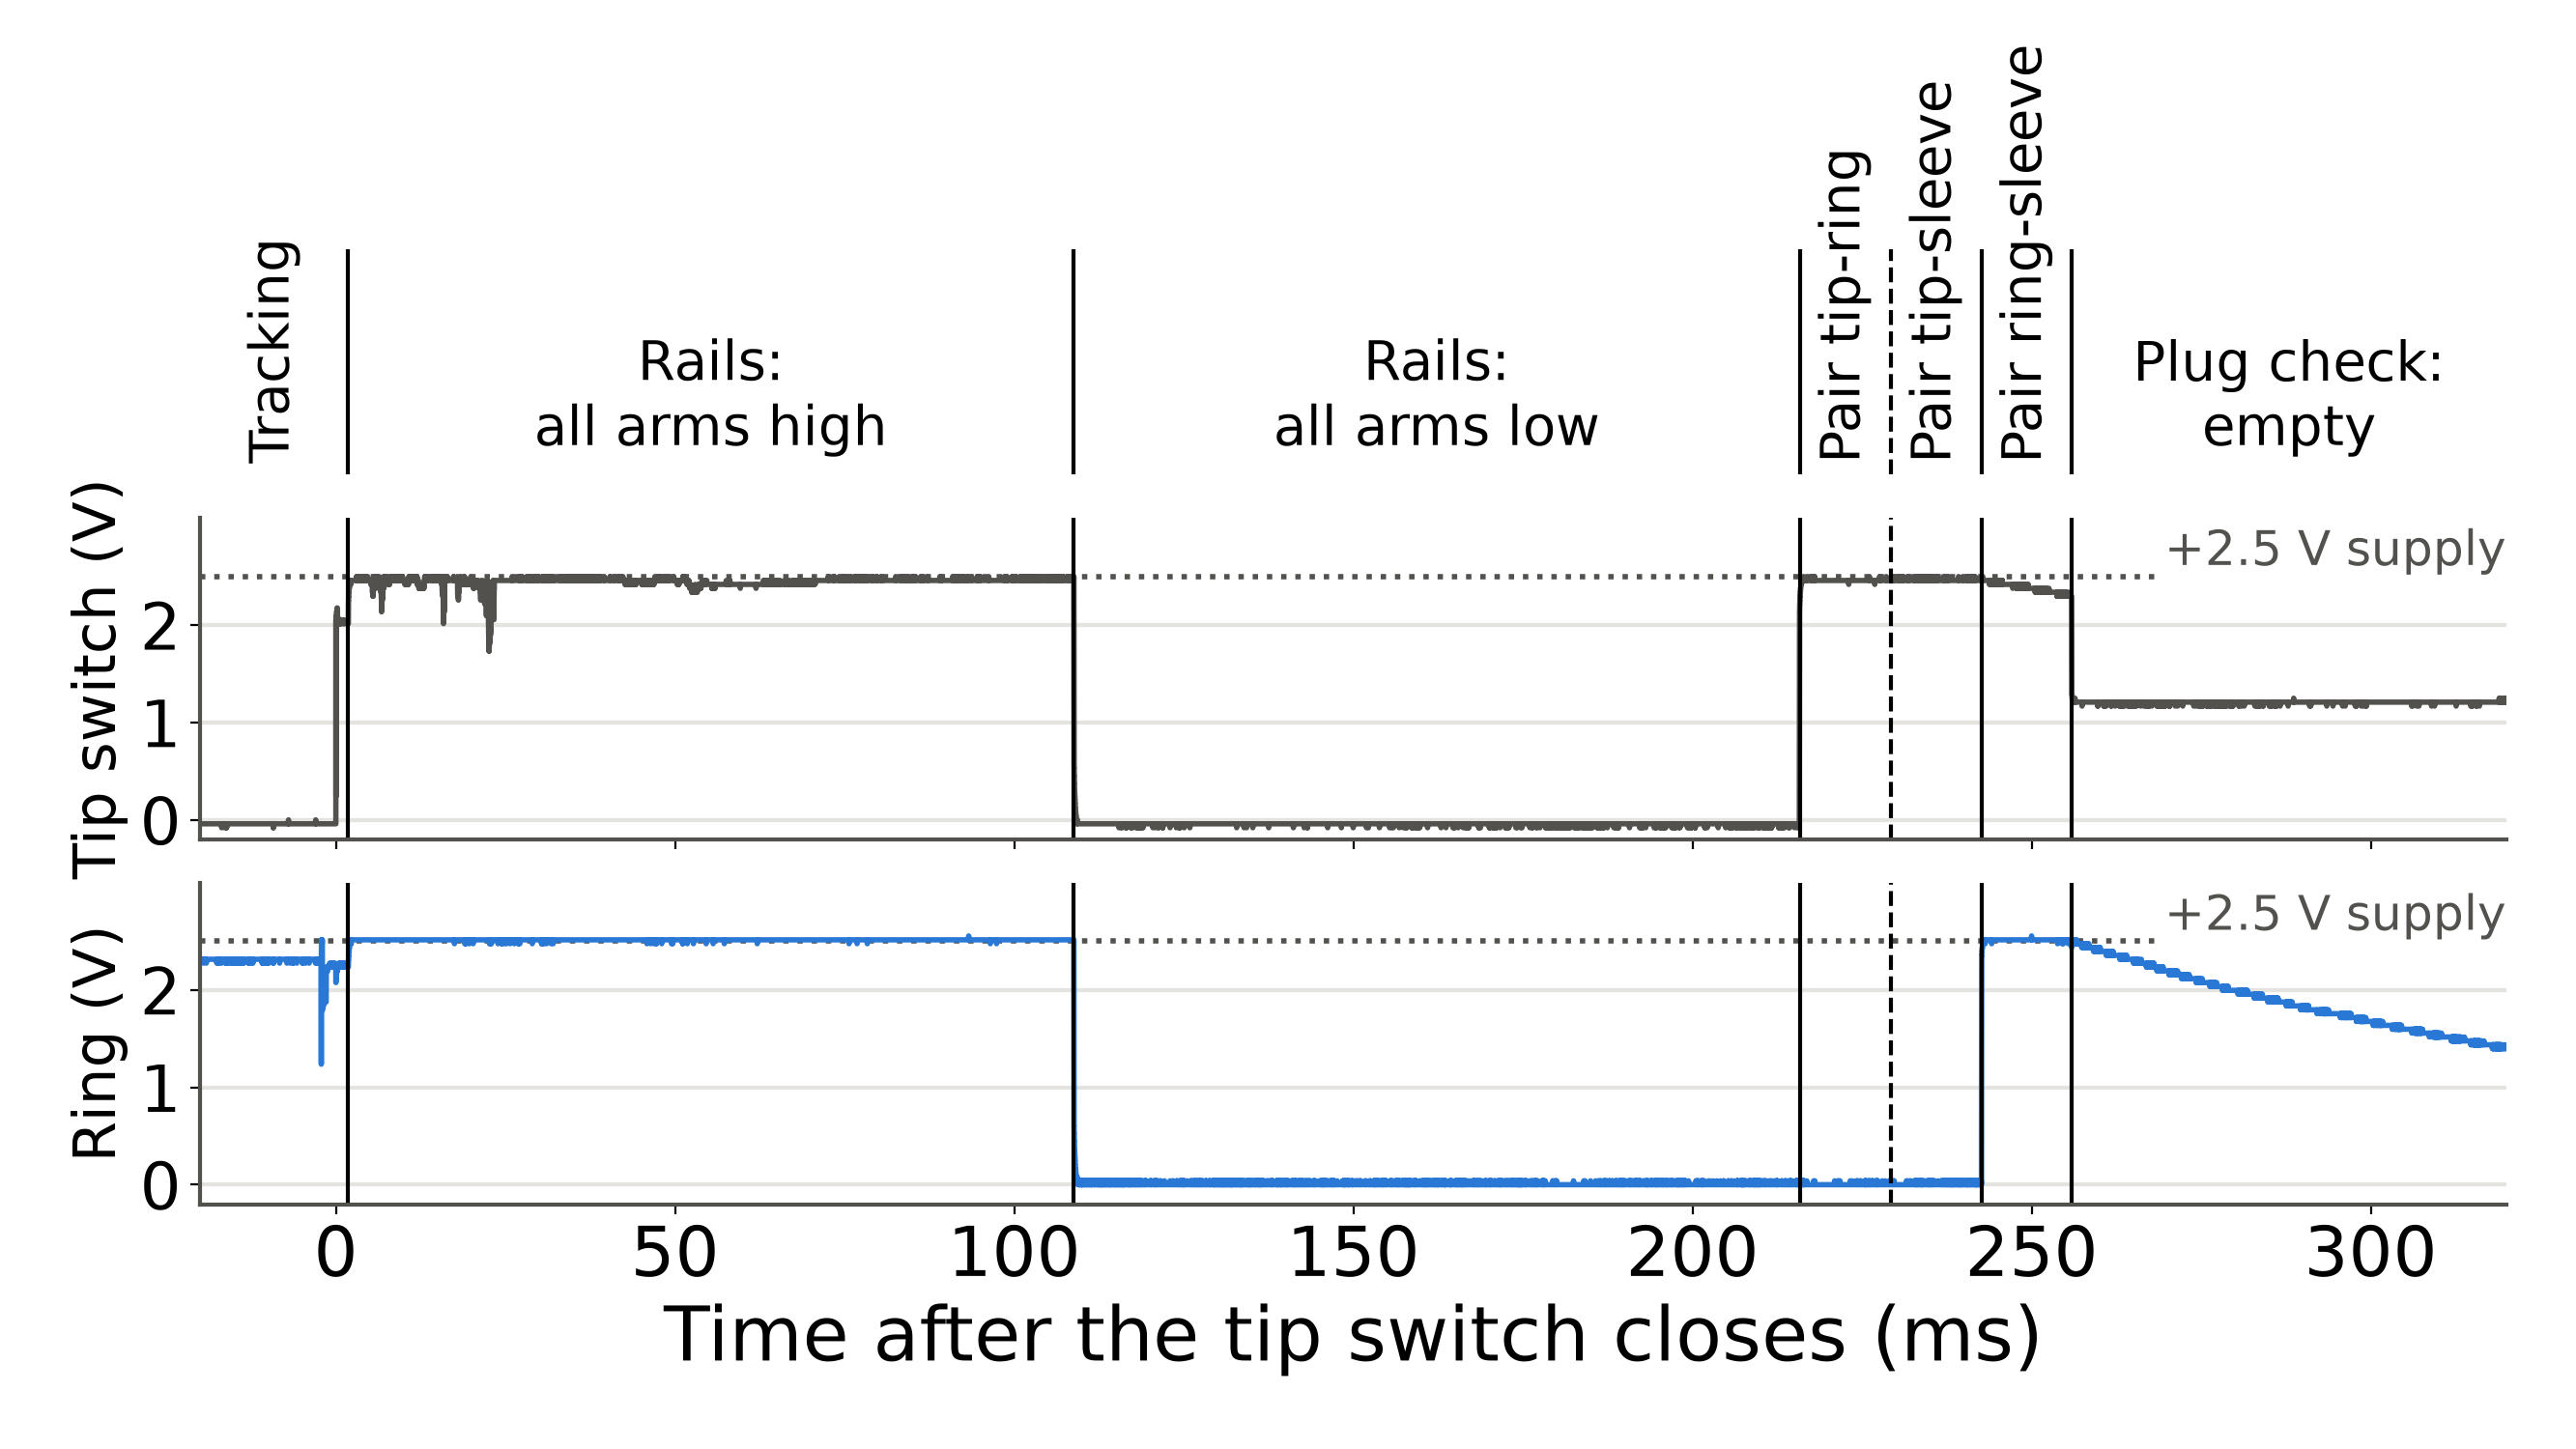
\includegraphics[width=\linewidth]{05-results/figures/unplug}
  \titledcaption{Unplug}{\scaffoldinline{Conditions (trigger on the tip switch closing); phases following, rails, three pairs, plug check; the dashed line is inferred. Capture \code{unplug1.csv}, the only run with a single solve.}}
  \label{fig:unplug}
\end{figure}

% !TEX root = ../main.tex

\section{Settling of a Floating Contact}
\label{sec:results-settling}

\scaffold{
  \textbf{Paragraph 1, the model under test.} \Cref{eq:settling} predicts that a floating contact charges with $\tau = (R_\mathrm{net} + R_\mathrm{f})\,C_\mathrm{f}$ and the firmware waits $2\tau$, at least \qty{1}{\milli\second}. A plug-in capture at \qty{0.5}{\micro\second} resolution contains such a step: in the second pair the ring switches from driven low to floating and charges through a pedal of about \qty{9.4}{\kilo\ohm}. A least-squares fit gives $\tau = \qty{190.6}{\micro\second}$ against $(9.4 + 10)\,\unit{\kilo\ohm} \times \qty{10}{\nano\farad} = \qty{194}{\micro\second}$ predicted. Only \qty{0.61}{\volt} of the \qty{1.71}{\volt} step follow the RC curve; the rest happens instantly. After the \qty{1}{\milli\second} minimum wait ($5.2\,\tau$) \qty{3.2}{\milli\volt} are missing, and the floating contact is read last in its pair, about \qty{9}{\milli\second} after the latch, so the error is negligible.
}

\scaffold{
  \textbf{Paragraph 2, latch edges.} A driven contact jumps by about \qty{91}{\percent} at the latch edge and settles with $\tau \approx \qty{110}{\micro\second} = (\qty{10}{\kilo\ohm} + \qty{1}{\kilo\ohm}) \times \qty{10}{\nano\farad}$, because the filter capacitor sits behind the \qty{10}{\kilo\ohm} resistor; the minimum wait covers five to nine of these time constants.
}

\begin{figure}[htbp]
  \centering
  \placeholderfigure{
    \textbf{Content.} Floating-contact step of the ring after the latch of the tip-sleeve pair for three networks (two equal resistors $R$ between ring and tip and between tip and sleeve, $R = \qty{4.7}{\kilo\ohm}$, \qty{47}{\kilo\ohm}, \qty{220}{\kilo\ohm}), each with its exponential fit; normalized time axis.
    \textbf{Focus.} Mark the firmware's wait (\qty{2.2}{\milli\second} while the network is still unknown) and the moment the ring is read (about \qty{10.5}{\milli\second} after the latch). Expected time constants: \qty{156}{\micro\second}, \qty{590}{\micro\second}, \qty{2.3}{\milli\second}; at \qty{220}{\kilo\ohm} about \qty{1}{\percent} (\qty{27}{\milli\volt}) of the step should still be missing when it is read, which is the case that tests the model. Correct the \qty{220}{\kilo\ohm} curve for the \qty{10}{\mega\ohm} probe load (about \qty{2}{\percent}).
    \textbf{How to obtain.} Channel~1 on SR\_LAT (TP2), trigger rising at \qty{1.65}{\volt}, single; channel~2 on the ring, 10X, bandwidth limit on; \qty{5}{\milli\second}/div, trigger at \qty{10}{\percent}, at least 500k points; plug in within \qty{30}{\second} of the previous unplug so that the first latch is the first pair. The captures \code{settling\_*.csv} in the archive are unusable: they triggered on the plug sliding in.
  }
  \titledcaption{Settling of a Floating Contact}{\scaffoldinline{Conditions, the three networks, measured and predicted time constants, and the meaning of the two marked moments.}}
  \label{fig:settling}
\end{figure}

\openquestion{Settling series}{
  The settling series with known resistors was postponed from the presentation to the report. Has it been measured with the corrected trigger? If not, either measure it or report only the single plug-in data point of paragraph~1.
}

% !TEX root = ../main.tex

\section{Update Rate}
\label{sec:results-update-rate}

\scaffold{
  \textbf{Paragraph 1, measurement.} The controller firmware logs the number of position updates per jack every \qty{5}{\second}. With one pedal on its ADC, \numrange{188}{189} updates per second were measured after the SPI changes of \cref{sec:update-rate} (168 before); about \qty{15}{\percent} of the readings are track-end checks. Present \cref{tab:update-rate} and compare with the 2.6 updates per second of the first firmware, a factor of about 70. Point out which rows are measured and which calculated.
}

\begin{table}[htbp]
  \centering
  \titledcaption{Update Rate per Pedal}{\scaffoldinline{State which values are measured (firmware log) and which calculated; jacks 1 and 2 share one ADC, jacks 3 and 4 the other.}}
  \label{tab:update-rate}
  \begin{tabularx}{\linewidth}{@{}>{\raggedright\arraybackslash}X ll@{}}
    \toprule
    \textbf{Situation} & \textbf{Updates per second} & \textbf{Origin} \\
    \midrule
    First firmware, full solves of all jacks & 2.6 & measured \\
    Full solves at \qty{819}{\hertz} & 5.8 & measured (sweep \qty{171}{\milli\second}) \\
    One pedal on its ADC, \qty{1}{\mega\hertz} SPI & 168 & measured \\
    One pedal on its ADC, \qty{4}{\mega\hertz} SPI & 188 to 189 & measured \\
    Two pedals on one ADC, or all four jacks & $\approx$ 95 & calculated \\
    \bottomrule
  \end{tabularx}
\end{table}

\scaffold{
  \textbf{Paragraph 2, reading time.} Present \cref{tab:spi-trim}: the SPI changes shortened a reading by about \qty{0.34}{\milli\second} without changing the noise or producing outlying codes; three conversion periods take \qty{3.66}{\milli\second}, so about \qty{0.35}{\milli\second} of overhead per reading remain.
}

\begin{table}[htbp]
  \centering
  \titledcaption{Reading Time Before and After the SPI Changes}{\scaffoldinline{Conditions: \qty{819}{\hertz}, pedal in jack~1 held still, 300 readings per configuration. Source: \code{docs/fast-tracking.md}.}}
  \label{tab:spi-trim}
  \begin{tabular}{@{}lrr@{}}
    \toprule
    & \textbf{\qty{1}{\mega\hertz}, \qty{50}{\micro\second} guard} & \textbf{\qty{4}{\mega\hertz}, \qty{10}{\micro\second} guard} \\
    \midrule
    Reading with channel change & \qty{4357}{\micro\second} & \qty{4021}{\micro\second} \\
    Reading on the same channel & \qty{4188}{\micro\second} & \qty{3985}{\micro\second} \\
    Wiper noise ($\sigma$) & \qty{442}{\micro\volt} & \qty{431}{\micro\volt} \\
    Outlying codes in 300 readings & 0 & 0 \\
    \bottomrule
  \end{tabular}
\end{table}

\openquestion{Rate with several pedals}{
  The rate with two pedals on one ADC (jacks 1 and 2, or 3 and 4) and with four pedals is calculated, not measured. Measure it with the firmware log if pedals are available, and say which jacks were used.
}

\openquestion{End-to-end latency}{
  The milestone plan listed the latency from a resistance change to the value arriving at the host. The measurement guide describes it (a GPIO toggled when the packet is handed to USB, plus a timestamping MIDI monitor on the host), but no data exists. Measure it or state that it was dropped and why.
}

% !TEX root = ../main.tex

\section{Pedal Types}
\label{sec:pedal-types}

\scaffold{
  \textbf{Paragraph 1, tested pedals.} Present \cref{tab:pedal-types}: which pedals were plugged in, on which cable, what the device identified and whether that is correct. Distinguish hardware tests from simulated ones (host tests of the jack monitor) explicitly in the table and the text.
}

\begin{table}[htbp]
  \centering
  \small
  \titledcaption{Identified Pedals}{\scaffoldinline{Explain the columns; \enquote{host test} marks cases verified only against the simulated jack. Pedal models to be added.}}
  \label{tab:pedal-types}
  \begin{tabularx}{\linewidth}{@{}>{\raggedright\arraybackslash}X l >{\raggedright\arraybackslash}X l@{}}
    \toprule
    \textbf{Pedal} & \textbf{Cable} & \textbf{Identified as} & \textbf{Verified on} \\
    \midrule
    Potentiometer, \qty{10.85}{\kilo\ohm}, wiper on tip & stereo & expression pedal (tracking), 0.09 closed to 1.0 open & hardware \\
    Potentiometer, about \qty{11.4}{\kilo\ohm}, wiper on ring, \qtyrange{1}{1.9}{\kilo\ohm} in the wiper lead & stereo & expression pedal (near-end case) & hardware \\
    Sustain switch & mono & switch & hardware \\
    Potentiometer & mono & not usable (track halves in parallel) & hardware \\
    Sustain switch & stereo & switch (open while released) & host test \\
    Two-wire rheostat & mono, stereo & rheostat & host test \\
    Dual footswitch & stereo & other (no value sent) & host test \\
    Cable without pedal & mono / stereo & released switch / open & host test \\
    \bottomrule
  \end{tabularx}
\end{table}

\scaffold{
  \textbf{Paragraph 2, the resistive wiper.} The second potentiometer pedal is the reason for the \qty{25}{\percent} wiper limit and the near-end class of \cref{sec:following}: its wiper arm measured \qty{8}{\percent} of the total at rest and up to \qty{15}{\percent} while moving, so with the original limit of \qty{10}{\percent} it was classified as \enquote{other} over most of its travel and tracked with the wrong wiper near both ends. Its wiper resistance does not affect the position, since the wiper carries no current while followed. Give the probable cause of the wiper resistance (a worn contact, or a series resistor such as a minimum-volume control, which some Boss and Roland pedals have \cite{nonlinearlabs2026pedals}).
}

\scaffold{
  \textbf{Paragraph 3, behaviour while plugging.} Name the transient cases observed on the hardware and handled: a plug noticed before it is fully seated (\cref{sec:results-recognition}); a stereo cable plugged into the jack first and into a potentiometer pedal afterwards, which is identified correctly since the stereo ring check (\cref{sec:jack-monitor}); repeated replugging at both end stops. Then the limits that remain by design (\cref{sec:following}): potentiometers need a stereo cable, a mono cable without a pedal reads as a released switch, a mono rheostat first reads as a potentiometer on its end stop, and a wiper guessed wrong at the ring-sleeve end stop is corrected once the pedal moves.
}

\openquestion{Pedal models and coverage}{
  Name the models of the pedals in \cref{tab:pedal-types} (and of the \qty{9.4}{\kilo\ohm} pedal in the oscilloscope captures, if it is a third one). Were a two-wire rheostat, a stereo sustain pedal or a dual footswitch ever tested on the hardware? Was a plug-cycle stress test made (repeated plugging, counting misdetections)?
}

% !TEX root = ../main.tex

\section{Requirement Review}
\label{sec:results-requirements}

\scaffold{
  Close the loop on the proposal \cite{benson2026proposal} and the evaluation plan of milestone~1 with \cref{tab:requirements}: one row per promise, the number or observation that settles it, and a status (met, partly met, not met, dropped). No prose beyond one introductory and one closing sentence; interpretation belongs to \cref{ch:discussion}.
}

\begin{table}[htbp]
  \centering
  \small
  \titledcaption{Requirements and Results}{\scaffoldinline{Explain the source of each requirement (P: proposal, M: milestone-1 evaluation plan) and the status values. Fill in the status column after the open measurements are decided.}}
  \label{tab:requirements}
  \begin{tabularx}{\linewidth}{@{}l >{\raggedright\arraybackslash}X >{\raggedright\arraybackslash}X l@{}}
    \toprule
    & \textbf{Requirement} & \textbf{Result} & \textbf{Status} \\
    \midrule
    P & Detect presence and wiring of a pedal automatically & plug detection and classification, \cref{sec:results-recognition,sec:pedal-types} & \scaffoldinline{?} \\
    P & Value linear to the pedal angle & ratiometric wiper reading, drive curve for nonlinear pots; linearity not measured & \scaffoldinline{?} \\
    P & Real time without perceptible latency & 188 updates/s, recognition 65 to \qty{95}{\milli\second} (about \qty{300}{\milli\second} with rail refresh) & \scaffoldinline{?} \\
    P & One to four TRS jacks & four jacks & \scaffoldinline{?} \\
    P & Class-compliant USB MIDI & USB MIDI 1.0 device, no driver & \scaffoldinline{?} \\
    P & Calibration of the channels with no pedal & rails measured per arm, refreshed after \qty{30}{\second} & \scaffoldinline{?} \\
    P & Digital filter against noise and contact bounce & hysteresis on the MIDI value; rheostat needs three readings; no moving average & \scaffoldinline{?} \\
    P & Optional DIN MIDI output & not implemented & \scaffoldinline{?} \\
    M & Power supply quality & below the 7-bit limit, \cref{sec:results-supply} & \scaffoldinline{?} \\
    M & SPI signal quality & \cref{sec:results-spi} & \scaffoldinline{?} \\
    M & Functional self-test & \cref{sec:results-self-test} & \scaffoldinline{?} \\
    M & Identification of known static networks & host tests; hardware with real pedals only & \scaffoldinline{?} \\
    M & Accuracy and linearity & \scaffoldinline{open question} & \scaffoldinline{?} \\
    M & End-to-end latency & \scaffoldinline{open question} & \scaffoldinline{?} \\
    \bottomrule
  \end{tabularx}
\end{table}

